\chapter{Microscopic Theory of Linear Isotropic Materials}
\setcounter{section}{1}
\section{Microscopic Theory for Dielectrics}
Considérons le cas d'un matériau linéaire et isotopique dans le champ de polarisation est donné
par $\vec{P} = \epsilon_0\chi\vec{E}$ où $\chi$ est la susceptibilité diélectrique.

\subsection{Static Electronic Polarisation}
Les électrons ont une faible masse $m_e$ mais une "grande" charge $e$. En présence d'un champ électrique
$\vec{E}$, les électrons subissent une force électrique
\begin{equation}
\vec F_E(x) = -e\vec E
\end{equation}
Les électrons d'un diélectriques sont toujours associés à des particules positives : ils sont liés à 
celles-ci par un potentiel électrique qui a un minimum : la position d'équilibre. Ce potentiel est 
approximativement parabolique
\begin{equation}
U_p(x) = \dfrac{a}{2}x^2\qquad\Rightarrow\qquad F_p(x) = -ax
\end{equation}
Dans un modèle statique, la position ne varie pas avec le temps. Elle peut être trouvée par équilibre
des forces $x= -eE/a$. On en tire le moment dipolaire et par la même occasion, la polarisation
\begin{equation}
p = -ex = \frac{e^2}{a}E\qquad\Rightarrow\qquad P=N_ep = \frac{N_ee^2}{a}E
\end{equation}
On en tire $\DS \chi = \dfrac{N_ee^2}{a\epsilon_0}$. En considérant que le potentiel inter-atomique à 
distance $d_a$ vaut l'énergie de liaison $U_b$, on trouve que $a=2U_b/d_a^2$ ce qui mène à
\begin{equation}
\chi = \dfrac{N_ee^2d_a^2}{2\epsilon_0U_b}
\end{equation}
Le moment dipolaire d'un atome/molécule est relié au champ électrique par la polarisabilité 
électronique statique ($\alpha_{e,s},\ [m^3]$) : $p_a=\alpha_{e,s}.\epsilon_0.E$. Avec $Z$ électrons,
on trouve
\begin{equation}
\alpha_{e,s} = \dfrac{Ze^2d_a^2}{2\epsilon_0U_b}
\end{equation}

\newpage
\subsection{Dynamic Electronic Polarisation}
Il s'agit du modèle de \textit{Drude-Lorentz}. On considère la seconde loi de Newton avec en plus de 
la force électrique, une force de rappel lié au potentiel et un amortissement proportionnel à la 
vitesse du nuage d'électron
\begin{equation}
m_e\dfrac{d^2x}{dt^2} = -eE-ax-2m_e\gamma\dfrac{dx}{dt}\qquad\Leftrightarrow\qquad
\dfrac{d^2x}{dt^2}+2\gamma\dfrac{dx}{dt}+\omega_0^2x=-\dfrac{e}{m_eE}
\end{equation}
où $\omega_0^2 = a/m_e = 2U_b/(m_ed_a^2)$ est la fréquence de résonance. En régime harmonique 
$e^{i\omega t}$ pour $x$ et $E$, on trouve
\begin{equation}
-\omega^2x+i2\gamma\omega x + \omega_0^2x = -\dfrac{e}{m_e}E\qquad\Leftrightarrow\qquad
x=-\dfrac{eE}{m_e(\omega_0^2-\omega^2+i2\gamma\omega)}
\end{equation}
Pour la polarisabilité électronique d'un atome de $Z$ électrons, on trouve
\begin{equation}
\alpha_s = \dfrac{Ze^2}{\epsilon_0m_e}\dfrac{1}{\omega_0^2-\omega^2+i2\gamma\omega}
\end{equation}
Il s'agit d'un phénomène de résonance à la fréquence $\omega_0$ alors que l’amortissement 
contribue à la partie imaginaire. Notons que la polarisabilité tend toujours vers zéro à haute
fréquence\footnote{Les électrons ne savent pas "suivre" le champ.} et statique aux basses
fréquences\footnote{Comme dans la théorie statique.}


\subsection{Quantum Mechanical Theory In-a-Nutshell for Electronic Polarisation}
La mécanique quantique nous apprend que les niveaux d'énergies sont bien définis, avec des différences
bien définies : pour se faire absorbé, un photon doit avoir une énergie très précise. Soit $\omega_{0i}$
correspondant à la différence d'énergie entre l'état excité $i$ et le fondamental. Chaque transition électronique possible conduit à une ligne d'absorption étroite autour de la fréquence
$\omega_{0i}$, c'est la signification physique du delta de Dirac ci-dessous (règle d'or de Fermi). Comme
on parle d'absorption, cela implique la la règle de Fermi est directement liée à la partie imaginaire de 
la polarisabilité. Après de longs calculs
\begin{equation}
\Im(\alpha_e) = \sum_i \dfrac{\pi e^2|P_{0i}|}{m_e^2\omega^2\epsilon_0}\delta (\omega-\omega_{0i})
\end{equation}
La partie imaginaire est liée à la partie réelle par les relations de Kramers-Kronig. Celles-ci nous disent
que dans le cas d'un système causal, elles ne sont pas indépendantes. On trouve alors
\begin{equation}
\Re(\alpha_e) = \sum_i\dfrac{2e^2|P_{0i}|}{m_e^2\omega^2\epsilon_0}\dfrac{\omega_{0i}}{\omega_{0i}^2-\omega^2}
\end{equation}
Avec la règle d'or de Fermi, on peut facilement calculer la partie imaginaire et avec Kramers-Kronig\footnote{
Pas demandé de connaître à l'examen, mais impressionné si on le démontre.} retrouver la partie réelle. On 
peut généraliser l'expression dans le cadre de l'amortissement (voir syllabus, (3.21)).




\newpage
\subsection{Ionic Polarisation}
	\begin{wrapfigure}[7]{l}{6cm}
	%\vspace{-5mm}
	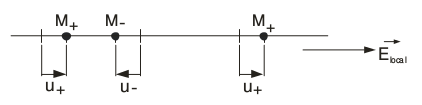
\includegraphics[scale=0.4]{ch3/image1.png}
	\captionof{figure}{ }
	\end{wrapfigure}
Lorsqu'un champ oscillant est présent, les ions vont bouger les uns par rapport aux autres. Considérons le
schéma ci-contre présentant des ions positifs et négatifs et un champ appliqué selon $\vec{1_x}$. En supposant
une force proportionnelle à la déviation de la position du centre d'équilibre des deux voisins, on trouve
\begin{equation}
M_-\dfrac{d^2u_-}{dt^2} = -2C(u_--u_+)-qE_{local}
\end{equation}
où $C$ est le facteur de proportionnalité entre la déviation et la force de rappel et le facteur 2 vient du fait
qu'il y a deux voisins. Pour un ion positif, on trouve 
\begin{equation}
M_+\dfrac{d^2u_+}{dt^2} = -2C(u_+-u_-)+qE_{local}
\end{equation}
Un champ local va exciter chaque type d'ion (local, qui est relié au global, nous y reviendrons). Par combinaison
linéaire, on trouve
\begin{equation}
M\dfrac{d^2u}{dt^2}+2Cu=qE_{local}
\end{equation}
où $u=u_+-u_-$ et où $M= M_+M_-/(M_++M_-)$ est la masse réduite. Par un couple d'ion, le moment dipolaire vaut
$qu$, la polarisabilité est alors donnée par 
\begin{equation}
\alpha(\omega) = \dfrac{q^2}{\epsilon_0(2C-M\omega^2)}
\end{equation}
Ce qui mène à la fréquence de résonance $\omega_{0,a} = \sqrt{\frac{2C}{M}}$. La fréquence de résonance sera
bien plus basse que celle causée par les électrons (en dessous du visible alors que pour ces-derniers c'était
au dessus), tout simplement car $M \gg m_e$.

\subsection{Orientation Polarisation}
Les molécules peuvent avoir des orientations "locales" aléatoire : en l'absence de champ électrique, la 
polarisation macroscopique est nulle. Si on applique $\vec{E}$, ils vont s'orienter dans la même direction
et la polarisabilité serait plus grande. Le processus est cependant assez lent (la molécule doit subir une
rotation) et se détruit facilement (par simple augmentation de la température). La physique statistique nous
donne une valeur que l'on peut associer à ce phénomène
\begin{equation}
\alpha_{as} = \frac{p^2}{3\epsilon_0k_BT}
\end{equation}
Ceci concerne les gaz et les liquides.



\subsection{The Field of Lorentz and the Local Field}
Nous avons précédemment introduit un champ \textit{local}, mais quel mécanisme peut lier ce-dernier au 
champ global? Le champ local peut être différent du global à cause des dipôles. Le champ externe interagit
avec ceux-ci et ils génèrent un second champ qui vient modifier le "champ perçu" par ces mêmes dipôles. Nous
allons ici suivre l'approche de Lorentz et calculer son champ moyen.
\newpage

	\begin{wrapfigure}[5]{r}{3cm}
	%\vspace{-5mm}
	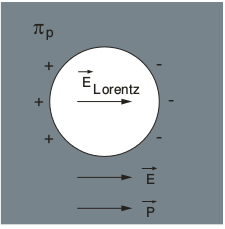
\includegraphics[scale=0.25]{ch3/image2.png}
	\captionof{figure}{ }
	\end{wrapfigure}
Nous allons calculer ce champ moyen en un point en construisant autour de ce point une sphère de rayon 
petit par rapport à l'échelle macroscopique, mais grande par rapport à l'échelle microscopique. A l'intérieur,
on va remplacer la matière continue par pleins de dipôles élémentaires. Le champ local est la somme de trois
contributions
\begin{enumerate}
\item Le champ $\vec{E}$ externe
\item Les dipôles présents
\item Les charges de surface sur la sphère (venant de la construction même de la sphère) : $\sigma_p = -
P\cos\theta$. Lorentz a calculé de que valait ce champ, il a trouvé
\begin{equation}
E_{\text{Lorentz}} = \dfrac{P}{3\epsilon_0}
\end{equation}
Il s'agit donc du champ généré par les charges de surface.
\end{enumerate}
Dans beaucoup de matériaux (si le cercle est centrée sur le point), la contribution des dipôles sera nulle. 
On trouve alors
\begin{equation}
E_{local} = E+\frac{P}{3\epsilon_0}
\end{equation}

\subsection{Clausius-Mosotti Relation}
Utilisons l'expression juste obtenue pour ré-écrire le moment dipolaire
\begin{equation}
p_i = \alpha_i\epsilon_0E_{local} = \alpha_i\epsilon_0\left(E+\dfrac{P}{3\epsilon_0}\right)
\end{equation}
Cette relation relie le force des dipôles au champ local. On peut en déduire le champ de polarisation
\begin{equation}
P = \sum_i N_i p_i = \sum_i N_i\alpha_i\epsilon_0\left(E+\dfrac{P}{3\epsilon_0}\right)
\end{equation}
L'équation est maintenant "fermée". On y voit une sorte de récurrence car le champ local dépend du champ de
polarisation : il faut connaître le 
champ de polarisation pour connaître le champ local puis utiliser ce dernier pour trouver le champ de
polarisation ! Ce qui est beau, c'est que l'on trouve une nouvelle expression pour la susceptibilité électrique
\begin{equation}
\chi_e = \frac{P}{\epsilon_0E}=\dfrac{\sum_i N_i\alpha_i}{1-\frac{1}{3}\sum_i N_i\alpha_i}
\end{equation}
Ce qui est important de comprendre c'est que le champ local défini la polarisabilité et qu'en sommant et 
fermant la relation obtenue on obtient celle-ci. La susceptibilité est donc donnée par la somme des 
polarisabilité divisée par une correction venant du champ local de Lorentz. \\

La loi de Clausius-Mosotti permet de réécrire $E_{local}$ (basée sur l'expression des cristaux cubiques) 
pour obtenir la \textbf{loi de Clausius-Mosotti}
\begin{equation}
\dfrac{\chi_e}{\chi_e+3}=\frac{1}{3}\sum_i N_i\alpha_i
\end{equation}
Avec cette définition de la suceptibilité, la relation de Lorentz devient
\begin{equation}
E_{\text{Local}} = \left(1+\dfrac{\chi_e}{3}\right)E
\end{equation}
L'important est - encore une fois - de voir d'où le problème vient : on travaille sur des effets macroscipique
mais résultant d'un champ local sommé au champ externe.


\subsection{General Dielectric Behaviour}
Reprenons les précédents résultats. La polarisation électronique se situe dans l'UV (une ou plusieurs 
résonances). La polarisation se situe (une ou plusieurs résonances)  dans l’infrarouge et la polarisation 
d'orientation à une fréquence critique dans les radio.
\begin{center}
	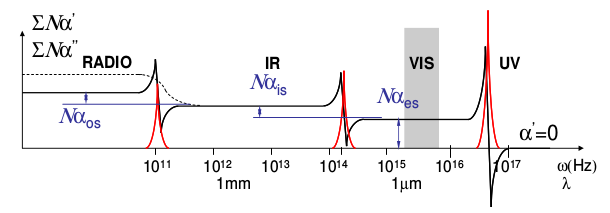
\includegraphics[scale=0.6]{ch3/image3.png}
	\captionof{figure}{Attention, les résonances montent d'abord puis elle descendent, pas l'inverse!}
\end{center}
On voit que les différentes résonances ne sont pas dans le visible. Cependant, le nombre de résonances "avant
et après" le visible influence la valeur "du visible" : les résonances ont une contribution indirectes. Pour
récapituler, $\alpha$ est la tendance à polariser une charge \textbf{unique} (ion, électron,\dots) alors que
$\chi$ est la tendance à polariser \textbf{tout} le matériau. La loi de Clausius-Mozotti donne la relation entre
$\alpha$ et $\chi$.


\section{Microscopic Theory for Conductors and Semiconductors}
Dans les dielectriques, la réaction de $E$ est décrite par $P$. Dans un conducteurs, par le courant $J$ car
les électrons sont libres de se mouvoir\footnote{"\textit{Le modèle de Drude est \textbf{vraiment à connaître}}".}.

\subsection{The 1D Drude Free-Electron Model for Metals}
Soit des ions à positions fixes et des électrons dans la bande de conduction : pas d'interactions entre les deux
espèces, mais les électrons accélèrent en présence de $\vec{E}$. Parfois, les $e^-$ collisionnent avec les ions
ou les impuretés. La probabilité de collision sur $dt$ est donnée par $dt/\tau$. Les collisions ne sont pas
élastiques, mais la vitesse après collision est dictée par la condition d'équilibre thermique. Sans $\vec{E}$, 
la vitesse moyenne des $e^-$ et donc $J$ est nul.\\

Soit $E(t)$ et un ensemble d'$e^-$ avec une position moyenne $x$. Négligeons la variation spatiale. L'impulsion
linéaire moyen $m\text{d}x/\text{d}t$ au temps $t+\text{d}t$ (où $dt\ll \tau$) est composé de deux contributions
\begin{enumerate}
\item La fraction des électrons qui voient leurs impulsions augmentées sous l'influence de la force $-eE$
\begin{equation}
\left(1-\dfrac{\text{d}t}{\tau}\right)
\end{equation}
\item La fraction $\text{d}t/\tau$ des électrons qui n'obtiennent pas d'impulsion à cause de la collision avec
un ion.
\end{enumerate}
L'impulsion moyenne en $t+\text{d}t$ devient alors
\begin{equation}
m\dfrac{\text{d}x}{\text{d}t}(t+\text{d}t) = \left(1-\dfrac{\text{d}t}{\tau}\right)\left(m\dfrac{\text{d}x}{
\text{d}t}(t)-eE(t)\text{d}t)\right)
\end{equation}
Ceci mène à l'équation de mouvement
\begin{equation}
m\dfrac{\text{d}^2x}{\text{d}t^2}=-\dfrac{m}{\tau}\dfrac{\text{d}x}{\text{d}t}-eE
\end{equation}
où l'on reconnaît un terme de \textit{damping} à droite. Notons qu'il y a \textbf{également} des électrons
liés dans un conducteurs, dans les basses couches. Sachant que $J = -Ne\dfrac{\text{d}x}{\text{d}t}$
\begin{equation}
\dfrac{\text{d}J}{\text{d}t} = -\dfrac{J}{\tau}+\dfrac{Ne^2}{m}E
\end{equation}
Ce qui devient, en régime harmonique $e^{i\omega t}$
\begin{equation}
J(\omega) = \dfrac{Ne^2\tau}{m(1+i\omega\tau)}E(\omega)
\end{equation}
Connaissant la loi d'Ohm
\begin{equation}
\sigma(\omega) = \dfrac{Ne^2\tau}{m(1+i\omega\tau)}
\end{equation}
Il s'agit de la \textbf{complex frequency dependant conductivity}. \\

Nous avions trouvé au chapitre 2
\begin{equation}
\epsilon = \epsilon_0\left(1+\chi-i\dfrac{\sigma}{\omega\epsilon_0}\right) = \epsilon_0\left(1+\chi+
\dfrac{Ne^2}{m\epsilon_0}\dfrac{1}{-\omega^2+i\omega/\tau}\right)
\end{equation}
Ceci est facile à interpréter si l'on 
remarque que $1/\tau$ est la fréquence de collision. A basse fréquence, la partie complexe de la constante
diélectrique deviant importante (par les relations de KK, cela va avoir une influence sur la partie réelle). Si en plus plus $\omega \gg 1/\tau$, le terme d'amortissement peut être
négligé et la courant d'électron libre contribue négativement à la constante diélectrique. La susceptibilité
équivalente due à la conduction ("plasma" idéal) est 
\begin{equation}
\chi_{\text{conduction}} = -\dfrac{\omega_p^2}{\omega^2}
\end{equation}
Qui devient $-1$ à la fréquence plasma $\omega_p = \sqrt{(Ne^2	)/(m\epsilon_0)}$.




\subsection{Cubic Crystals}
Le reste du chapitre n'est pas pour l'examen.






























